\documentclass[12pt]{article}

\usepackage{sigsam, bm, bbm, amsmath}
\usepackage{amssymb,stmaryrd}
\usepackage{color}
\usepackage{hyperref}
\usepackage[american]{babel}
\usepackage[utf8]{inputenc}
\usepackage[OT1]{fontenc}

\usepackage{algorithm}
\usepackage{algorithmic}
\renewcommand{\algorithmicrequire}{\textbf{Input:}}
\renewcommand{\algorithmicensure}{\textbf{Output:}}

\usepackage{tikz}

% Tikz style

\tikzset{round/.style={circle, draw=black, very thick, scale = 0.7}}
\tikzset{arrow/.style={->, >=latex}}
\tikzset{dashed-arrow/.style={->, >=latex, dashed}}

\usetikzlibrary{positioning}
\usetikzlibrary{calc}
\usetikzlibrary{decorations.pathreplacing}
\usetikzlibrary{matrix}
\usetikzlibrary{intersections}
\usetikzlibrary{backgrounds}
\usetikzlibrary{fit}
\usetikzlibrary{arrows}

% Math Operators

\DeclareMathOperator{\Card}{Card}
\DeclareMathOperator{\Gal}{Gal}
\DeclareMathOperator{\Id}{Id}
\DeclareMathOperator{\Img}{Im}
\DeclareMathOperator{\Ker}{Ker}
\DeclareMathOperator{\Minpoly}{Minpoly}
\DeclareMathOperator{\Mod}{mod}
\DeclareMathOperator{\Ord}{Ord}
\DeclareMathOperator{\ppcm}{ppcm}
\DeclareMathOperator{\Tr}{Tr}
\DeclareMathOperator{\Vect}{Vect}

% Shortcuts

\newcommand{\dE}{\partial(E)}
\newcommand{\dF}{\partial(F)}
\newcommand{\dG}{\partial(G)}
\newcommand{\diff}{\mathop{}\!\mathrm{d}}
\newcommand{\eg}{\emph{e.g. }}
\newcommand{\emb}{\hookrightarrow}
\newcommand{\embed}[2]{\phi_{#1\hookrightarrow#2}}
\newcommand{\ent}[2]{[\![#1,#2]\!]}
\newcommand{\ie}{\emph{i.e. }}
\newcommand{\ps}[2]{\left\langle#1,#2\right\rangle}
\newcommand{\FF}{\mathbb{F}}



\def\Q {\ensuremath{\mathbb{Q}}}
\def\Z {\ensuremath{\mathbb{Z}}}
\def\F {\ensuremath{\mathbb{F}}}
\def\Tr {\ensuremath{\mathrm{Tr}}}

\def\M {\ensuremath{\mathsf{M}}}

\newcommand{\todo}[1]{\textcolor{red}{TODO: #1}}

\newtheorem{Def}{Definition}
\newtheorem{Theo}{Theorem}
\newtheorem{Prop}{Proposition}
\newtheorem{Lemma}{Lemma}

\issue{TBA}
\articlehead{TBA}
\titlehead{Lattices of compatibly embedded finite fields}
\authorhead{Luca De Feo, Hugues Randriambololona, Édouard Rousseau and Éric Schost}
\setcounter{page}{1}

\title{Lattices of compatibly embedded finite fields}
\author{Luca De Feo\footnote{
    Université de Versailles and Inria, Paris Saclay,
    \url{luca.de-feo@uvsq.fr}
  },
  Hugues Randriambololona\footnote{
    Télécom ParisTech,
    \url{randriam@telecom-paristech.fr}
  },
  Édouard Rousseau\footnote{
    Télécom ParisTech and Université de Versailles,
    \url{edouard.rousseau@telecom-paristech.fr}
  },
  Éric Schost\footnote{
    University of Waterloo
    \url{eshost@uwaterloo.ca}
  }
}

\begin{document}
\maketitle

Finite fields are widely used in mathematics and their applications. They are
often the building block of more complicated algebraic structure used in
cryptology or coding theory. As a
consequence, several computer algebra systems or libraries have been written in
order to work in arbitrary finite fields. Among them, we find
Magma~\cite{Magma}, Sage~\cite{Sagemath}, Flint~\cite{Flint}, NTL~\cite{NTL} or
PARI~\cite{Pari}. Many problems require not only to work in a given finite field
$K$, but also in finite extensions of $K$, as represented in
Figure~\ref{fig:alg-closure}, that are again finite fields, or in
the algebraic closure of $K$. In particular, it is desirable to be able to
freely \emph{move} from a field to a subfield or an extension.

Given two finite fields $E$ and $F$ with cardinalities $\#E=p^{m}$ and
$\#F=p^{n}$, we know that $E$ can be embedded in $F$ if and only if $m\,|\,n$.
In other words, $E$ is in that case isomorphic to a subfield $E'\subset F$ of
$F$ with
cardinality $\#E'=p^{m}$. There are
$m=[E:\mathbb{F}_p]=\#\Gal(E/\mathbb{F}_p)$ disctinct embeddings from $E$ to
$F$ (the degree of $E$ over $\mathbb{F}_p$ will also be denoted by
$\partial(E)$). Indeed, the Galois group of the extension $E$ over
$\mathbb{F}_p$ acts
on the embeddings and, given two different embeddings $\embed{E}{F}$ and
$\embed{E}{F}'$ and an element $x\in E$, the images $\embed{E}{F}(x)$ and
$\embed{E}{F}'(x)$ must be conjugate. There is no canonical
embedding from $E$ to $F$. Furthermore, the proof of the fact that $E$ can be
embedded in $F$ if and only if $\dE\,|\,\dF$ does not give an efficient
algorithm. Finding such an algorithm is an interesting problem, and there exists
a variety of solutions, see for example the survey paper~\cite{BDDFS17}.

\begin{figure}
  \centering
  \tikzset{
        dotstyle/.style={circle, inner sep = 1.2pt, outer sep = 4pt, fill =
        gray},
        edgetower/.style={thick},
        edgecomp/.style={thick, lightgray}
          }
  \begin{tikzpicture} [scale = 0.8] %, every node/.style={inner sep = 2pt, scale=0.8}]
    \coordinate (T2) at (-2, 0.5);
    \node (Fp) at (0, 0) {$\FF_p$};
    \node (Fp2) at ($(Fp) + (T2)$) {$\FF_{p^2}$};
    \node (Fp4) at ($(Fp2) + (T2)$) {$\FF_{p^4}$};
    \node (Fp2l) at ($(Fp4) + (T2)$) {};% {$\FF_p^{(2)}$};
    % ---------------------
    \coordinate (T3) at (-0.7, 2);
    \node (Fp3) at ($(Fp) + (T3)$) {$\FF_{p^3}$};
    \node (Fp9) at ($(Fp3) + (T3)$) {$\FF_{p^9}$};
    \node (Fp3l) at ($(Fp9) + (T3)$) {};% {$\FF_p^{(3)}$};
    % ---------------------
    \coordinate (T5) at (0.7, 2);
    \node (Fp5) at ($(Fp) + (T5)$) {$\FF_{p^5}$};
    \node (Fp25) at ($(Fp5) + (T5)$) {$\FF_{p^{25}}$};
    \node (Fp5l) at ($(Fp25) + (T5)$) {};% {$\FF_p^{(5)}$};
    % ---------------------
    \coordinate (Tl) at (2, .5);
    \node[blue] (Fpl) at ($(Fp) + (Tl)$) {$\FF_{p^\ell}$};
    \node[blue] (Fpl2) at ($(Fpl) + (Tl)$) {$\FF_{p^{\ell^2}}$};
    \node[blue] (Fpll) at ($(Fpl2) + (Tl)$) {};% {$\FF_p^{(\ell)}$};
    % ---------------------
    \node[dotstyle] (dot1) at ($(Fp2) + (Fp3) - (Fp)$) {};
    \node[dotstyle] (dot2) at ($(Fp4) + (dot1) - (Fp2)$) {};
    \node[dotstyle] (dot3) at ($(Fp2) + (Fp5) - (Fp)$) {};
    \node[dotstyle] (dot4) at ($(Fp3) + (Fp5) - (Fp)$) {};
    \node[dotstyle] (dot5) at ($(Fp3) + (Fpl) - (Fp)$) {};
    \node[dotstyle] (dot6) at ($(Fp5) + (Fpl) - (Fp)$) {};
    \node[dotstyle] (dot7) at ($(Fpl2) + (dot6) - (Fpl)$) {};
    % ---------------------
    \draw 
    (Fp) 
    edge[edgetower] (Fp2)
    edge[edgetower] (Fp3)
    edge[edgetower] (Fp5)
    edge[edgetower, blue] (Fpl)
    (Fp2)
    edge[edgetower] (Fp4)
    edge[edgecomp] (dot1)
    (Fp4)
    edge[edgetower, dotted] (Fp2l)
    edge[edgecomp] (dot2)
    (dot1)
    edge[edgecomp] (dot2)
    (Fp3)
    edge[edgetower] (Fp9)
    edge[edgecomp] (dot1)
    edge[edgecomp] (dot4)
    (Fp9)
    edge[edgetower, dotted] (Fp3l)
    (Fp5)
    edge[edgetower] (Fp25)
    edge[edgecomp] (dot4)
    edge[edgecomp] (dot6)
    (Fp25)
    edge[edgetower, dotted] (Fp5l)
    (Fpl)
    edge[edgetower, blue] (Fpl2)
    edge[edgecomp] (dot6)
    (Fpl2)
    edge[edgetower, blue, dotted] (Fpll)
    edge[edgecomp] (dot7)
    (dot3)
    edge[edgecomp] (Fp2)
    edge[edgecomp] (Fp5)
    (dot5)
    edge[edgecomp] (Fp3)
    edge[edgecomp] (Fpl)
    (dot6)
    edge[edgecomp] (dot7);
  \end{tikzpicture}
  \caption{Extensions of $\mathbb{F}_p$.}
  \label{fig:alg-closure}
\end{figure}


Additionaly, we want the embeddings to be compatible. Given three finite 
fields $E$, $F$, and $G$, such that $\dE\,|\,\dF$ and $\dF\,|\,\dG$, and three 
embeddings $\embed{E}{F}$, $\embed{F}{G}$, and $\embed{E}{G}$, we say that the
embeddings are \emph{compatible} if 
\[
  \embed{E}{G}=\embed{F}{G}\circ\embed{E}{F}.
\]
In other words, we want the diagram of Figure~\ref{fig:compatibility} to
commute. In the context of a computer algebra system, this condition is
important in order to give the user coherent answers when performing operations
in different fields. This is the case when computing in the algebraic closure of a
finite field, because the ambient field may change often. There are also
applications in isogeny-based or pairing-based cryptography.
We note $E\emb F$ if $E$ is explicitly embedded in $F$, \ie if
we have computed an embedding $\embed{E}{F}$.
\begin{figure}
  \centering
    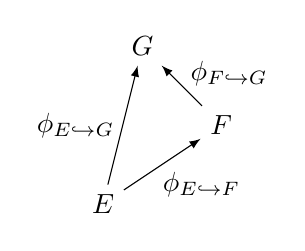
\begin{tikzpicture}
      \node (E) at (0, 0) {$E$}; 
      \node (F) at (1.5, 1) {$F$}; 
      \node (G) at (0.5, 2) {$G$}; 

      \draw[arrow] (E) -- (F);
      \draw[arrow] (E) -- (G);
      \draw[arrow] (F) -- (G);

      \node (f12) at (1.25, 0.25) {$\embed{E}{F}$};
      \node (f13) at (-0.35, 1) {$\embed{E}{G}$};
      \node (f23) at (1.6, 1.65) {$\embed{F}{G}$};
    \end{tikzpicture}

  \caption{Embeddings between finite fields.}
  \label{fig:compatibility}
\end{figure}

\paragraph{Compatibility}

Compatibility can be achieved using \emph{Conway polynomials}~\cite{Parker90, HL98}, a set $\left\{
P_d \right\}_{d\in D}$ of
irreducible polynomials over $\mathbb{F}_p$ such that any root $\beta_d$ of
$P_d$ is primitive in $\mathbb{F}_{p}[X]/(P_d(X))\cong \mathbb{F}_{p^d}$ and
such that if $d_1, d_2\in D$ and $d_1|d_2$, then
$N_{\mathbb{F}_{p^{d_2}}/\mathbb{F}_{p^{d_1}}}(\beta_{d_2})$ is a root of
$P_{d_1}$, where $N_{\mathbb{F}_{p^{d_2}}/\mathbb{F}_{p^{d_1}}}$ denotes
the norm of $\mathbb{F}_{p^{d_2}}$ over $\mathbb{F}_{p^{d_1}}$. A compatible
embedding of $\mathbb{F}_{p^{d_1}}$ in $\mathbb{F}_{p^{d_2}}$ is then obtained
by sending $\beta_{d_1}$ to $\beta_{d_2}^k$, with $k=(p^{d_2}-1)/(p^{d_1}-1)$.
By adding a minimality condition with respect to some ordering, this provides a
way of constructing standardized finite field extensions. However Conway polynomials
are hard to compute, so in practice this technique can only be used with rather
small fields.

Bosma, Cannon and Steel suggested another scheme~\cite{BCS97} in which they
give an axiomatic characterization of a lattice of compatibly embedded finite
fields. Their method does not require any precomputation and enables to work in
any user-defined finite field. However, embedding a new finite field requires
polynomial factorization and leads to a quadratic cost in the extension degree.
Given a pair $\mathfrak L=(L, \Phi)$, where
$L$ is a set of finite fields and $\Phi$ is a set of embeddings between
elements of $L$, we say that $\mathfrak L$ is a \emph{lattice of compatibly
embedded finite fields} if
\begin{enumerate}
  \item[CE1] (unicity) for each pair $(E, F)$ of elements in $L$, there exists
    at most one corresponding embedding $\embed{E}{F}\in\Phi$.
  \item[CE2] (reflexivity) For each $E\in L$, the identity map
    $\Id_E=\embed{E}{E}$ is in $\Phi$.
  \item[CE3] (prime subfield) There is exactly one $P\in L$ such that $\partial
    (P) = 1$, and for all $F\in L$, there exists $\embed{P}{F}\in\Phi$
  \item[CE4] (invertibility) If $E\emb F$ and $\dE=\dF$, then $F\emb E$ and
    $\embed{F}{E}=\embed{E}{F}^{-1}$.
  \item[CE5] (transitivity) For any triple $(E, F, G)$ of elements in $L$, if $E\emb
    F\emb G$ then $E\emb G$ and
    $\embed{E}{G}=\embed{F}{G}\circ\embed{E}{F}$.
  \item[CE6](intersections) For each $E, F, G\in L$ such that $F\emb G$ and
    $E\emb G$, there exists $S\in L$ such that $\partial(S)=\gcd(\dE, \dF)$
    and $S\emb E$, $S\emb F$.
\end{enumerate}

Under those conditions, we can prove~\cite{BCS97} that we are able to add a
finite field in
$L$ or an embedding that is not yet in $\Phi$ without altering the compatibility
of the lattice $\mathfrak L$.

\paragraph{Our contribution}

We implemented Bosma, Canon and Steel framework using Nemo/Flint~\cite{Nemo,
Flint} and following conditions CE1 to CE6. These
conditions are, for most of them, very natural. The condition CE3 is
technical and does not imply any work in our implementation because
finite fields elements in Nemo/Flint are represented by
polynomials over $\mathbb{F}_p$, so the embedding of $\mathbb{F}_p$ into an
extension is trivial. Finally, condition
CE6 ensures that the implicit isomorphisms between subfields are made
explicit. In order to meet this last condition, when embedding a finite field
$F$ in $G$, for each subfield $S$ of $G$, we check that the finite field $S\cap F$ is 
embedded in $S$ and $F$, and if not, we embed it. If there is not
any finite field of degree $d=\gcd(\partial(S), \dF)$, we compute an
arbitrary finite field $I$ of degree $d$ using Flint
and we embed $I$ in $S$ and $F$. This results in a recursive call to our
embedding algorithm, so the complexity of the operation might explode at that step.

Our code is available as an experimental branch of
Nemo\footnote{\url{https://github.com/erou/Nemo.jl/tree/embeddings}}, that is
itself based on an experimental branch of
Flint\footnote{\url{https://github.com/defeo/flint2/tree/embeddings}}. Critical
routines (\eg polynomial factorization, matrix computations) are written in C and
computed by Flint, whereas high level tasks (\eg checking conditions CE5 and CE6) are
written in Julia using Nemo. Our goal is to first include the C code inside the
standard Flint library and then the Julia code in Nemo.
With our experimental code, it is possible to define arbitrary finite fields and
to compute compatible embeddings between them, it is also possible to compute a ``projection'' of a
field to a subfield: \ie a map that sends an element to its inverse image when
the element is in the subfield, and throw an error otherwise. All these
computations are automatic and invisible to the user, except if he or she wants
to work with the maps themselves.

\paragraph{Future work}

The code has yet to be optimised: condition CE5 could be droped and the
``transitive closure'' of our lattice would be computed only if needed by the
user. Some technical computations inside the framework could also be optimised
using non-naive algorithms or by being written in C instead of Julia. Finally,
the embedding algorithm used by Bosma,
Canon and Steel (the naive algorithm) is not optimal either. Replacing the naive
algorithm by more sophisticated algorithm requires both theoretic work and some
new implementations. An important question is whether a ``standardized''
construction can be found for these algorithms, similar to the one obtained
using Conway polynomials. Contrary to Bosma, Canon and Steel framework, Conway
polynomials also permit to simply obtain the generator of a field from the
generator of another field using norms. We aim to be able to do the same thing,
by memorizing a little more than the generators of our finite fields.

\bibliographystyle{plain}
\bibliography{erou}

\end{document}


% Local Variables:
% ispell-local-dictionary:"american"
% End:

%  LocalWords:  isomorphism
